%do not change the documentclass
\documentclass[10pt, a4paper]{collection-edmi}
\usepackage{caption}

\usepackage[utf8]{inputenc}

\begin{document}
%%%%%%%%%%%%%%%%%%%%%%%%%%%%%%%%%%%%%%%%%%%%%%%%%%%%%%%%%%%%%%%%%%%%%%%%%%%%%%%%
% Custom commands must be defined HERE

%%%%%%%%%%%%%%%%%%%%%%%%%%%%%%%%%%%%%%%%%%%%%%%%%%%%%%%%%%%%%%%%%%%%%%%%%%%%%%%%
% The article title
\title{A cognitively plausible architecture for a metacognitive agent}
% Author
\author{Baptiste PESQUET}
% Direction
\direction{
    Directeur: Frédéric ALEXANDRE
}

%Institutions. \imbinria, \labriinria, \imb, \labri are available.
\institution{\labriinria}
% Print the title
\maketitle
% \thispagestyle{firstpage}

%%%%%%%%%%%%%%%%%%%%%%%%%%%%%%%%%%%%%%%%%%%%%%%%%%%%%%%%%%%%%%%%%%%%%%%%%%%%%%%%
% Abtract
\begin{abstract}
Human cognition stands out through its capacity for metacognition — the ability to monitor, evaluate, and control one's own mental processes. While recent advances in artificial intelligence have given impressive results in decision-making and learning, existing approaches still fall short of replicating the flexibility and self-awareness that characterize human cognition. Drawing from research at the intersection of experimental psychology, computational neuroscience, and reinforcement learning, we propose a cognitively plausible architecture for a metacognitive artificial agent. To evaluate this architecture, we introduce a dedicated object sorting task inspired by a human-robot collaboration scenario, in which the agent must learn to maximize reward under environmental uncertainty. Comparisons with standard reinforcement learning algorithms and the metacognitive architecture are ongoing. This work lays the groundwork for artificial agents capable of more autonomous, flexible, and self-regulated behavior.
\end{abstract}

%%%%%%%%%%%%%%%%%%%%%%%%%%%%%%%%%%%%%%%%%%%%%%%%%%%%%%%%%%%%%%%%%%%%%%%%%%%%%%%%
% Content
\begin{content}
\section{Motivation}
Decision-making and learning are two hallmarks of cognition, and mutually influential processes \cite{mileticNewModelDecision2021}. Both are key skills to adapt to one's environment and reach one's goals. Advances in artificial intelligence (AI), particularly in large language models \cite{radfordLLM} and reinforcement learning (RL) systems \cite{suttonBartoRL}, have narrowed the gap between artificial and human aptitudes in these fields. Yet, human cognition is uniquely characterized by several traits: ability to generalize from few examples, adaptability to uncertainty and changes in the environment, capacity to define one's own goals and explain one's behavior, and ability to evaluate and control one's mental processes (\textit{metacognition}). Despite recent progress \cite{weiCoTreasoning2024} \cite{botvinickRLfastslow}, current AI systems mostly excel at reactive, implicit decision-making and struggle to replicate the flexibility of human cognition.

Inspired by research in experimental psychology and cognitive modeling, we propose an architecture for an artificial agent augmented with metacognitive abilities. Its decision-making and learning abilities are evaluated through a novel object sorting task.

\section{Related work}

A decision is a deliberative process that results in the commitment to a categorical proposition \cite{goldNeuralBasis2007}. Many cognitive models of decision-making envision a decision as an accumulation-to-threshold operation. These are known as \textit{sequential sampling models} or \textit{evidence accumulation models} (EAM) \cite{forstmannSSM2016}. Another class of models combines reinforcement learning and evidence accumulation in order to describe the mutual interactions between learning and decision-making \cite{mileticNewModelDecision2021}.

The framework of reinforcement learning, in which an agent learns to gradually refine its behavior to maximize a cumulative reward, draws on foundational ideas from behavioral psychology. Similarities at both the behavioral and computational levels have been reported with reactive decision making in animals \cite{suriNNDopamine1999}. The addition of Deep Learning techniques has given birth to powerful new methods in the field \cite{mnihDQN2015}. Another line of research augments RL with episodic or working memory systems, extending its use to non-Markovian contexts \cite{zilliModelingWMEM2008}. Other approaches try to give agents the ability to choose actions at different time scales, paving the way for deliberative decision-making and goal-directed behavior \cite{stolleOptionsRL2002}, \cite{baconOptionCritic2016}.

Metacognition, the capacity to reflect on, evaluate, and control one's own mental functions, is a defining trait of natural cognition. To monitor its cognitive processes, the brain performs \textit{confidence judgments}, quantifying the degree of certainty associated with its decisions. Some cognitive models of sequential decision-making account for confidence as the difference between accumulators for each alternative. A larger gap is associated with a higher degree of confidence, reflecting a more robust decision. Furthermore, this approach is biologically grounded \cite{KepecsDecisionConfidence2008}. Other models use confidence as the switch mechanism between different behavior rules \cite{koechlinPROBE2012}.

\section{Methodology}

\subsection{Proposed architecture}

Taking into account the previous literature on confidence and human decision-making, we designed a model for an artificial agent using a cognitively plausible architecture for learning and decision-making.

The decision module uses evidence accumulation to select the object to aim for, based on the current perception of the environment. This evidence accumulation is driven by the difference in Q-values between the different possible actions, which are refined through reward prediction errors.

The metacognitive module uses the difference between accumulators to compute the confidence associated to each decision. Confidence is then used to tune the decision process by updating the hyperparameters of the decision process: rate of evidence accumulation and threshold to reach a decision.

\subsection{Test environment}

In order to compare agent architectures, a dedicated task has been designed from the ground up. It is a simplified version of the experimental protocol set up for the COURRIER ANR project in which we participate: two agents represented as robotic arms must pick and place a series of objects moving in front of them \ref{fig:collabsort_task}. Rewards for picking an object are agent-specific and depend on object properties (shape and color). They may evolve between episodes, introducing volatility for agents. Collisions between arms are penalized. 

One of the agents is deterministic and selfish. It has access to all environment information, knows the initial object reward structure and uses hardcoded behaviorial rules to pick objects. The other agent is used to compare different cognitive architectures. It has to learn to maximize its cumulative reward while adapting to the other agent's behavior and to uncertainties in the environment.

The task is implemented in Python as a Gymnasium environment. Its source code is available online \footnote{https://github.com/bpesquet/gym-collabsort}.

\begin{floating}
    \centering
    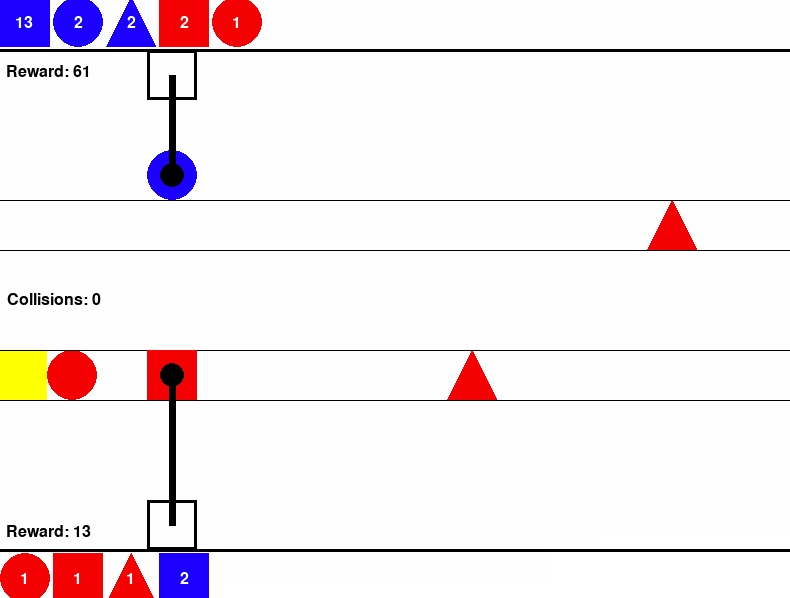
\includegraphics[width=\textwidth]{./img/collabsort_demo.jpg}
    \captionof{figure}{The collaborative object sorting task used as a test environment. Each agent is represented by a vertically moving arm extending from a square base and terminated by a round gripper. It can pick and place objects moving from right to left on two treadmills. The agent as the top is deterministic. The one at the bottom implements different cognitive architectures.}
    \label{fig:collabsort_task}
\end{floating}

\subsection{Preliminary results}

The environment has been instrumented to evaluate different performance metrics. Since the idea is to compare our novel cognitive architecture with existing solutions, an agent has been developed that implements a classic Deep Q-Learning algorithm \cite{mnihDQN2015} as a benchmark. Its results (\ref{fig:collabsort_results}) demonstrate an ability to learn the task structure. However, its behavior (observable when launching another simulation with the trained agent) remains far from perfect, with too few picked objects compared with the other, hardcoded agent. Nevertheless, these results constitute a good baseline.

Work is underway to implement other reinforcement learning algorithms (Actor-Critic, PPO) and, more importantly, compare the proposed cognitive architecture against them. The source code of all experiments is available online \footnote{https://github.com/bpesquet/collabsort-agent}.

\begin{floating}
    \centering
    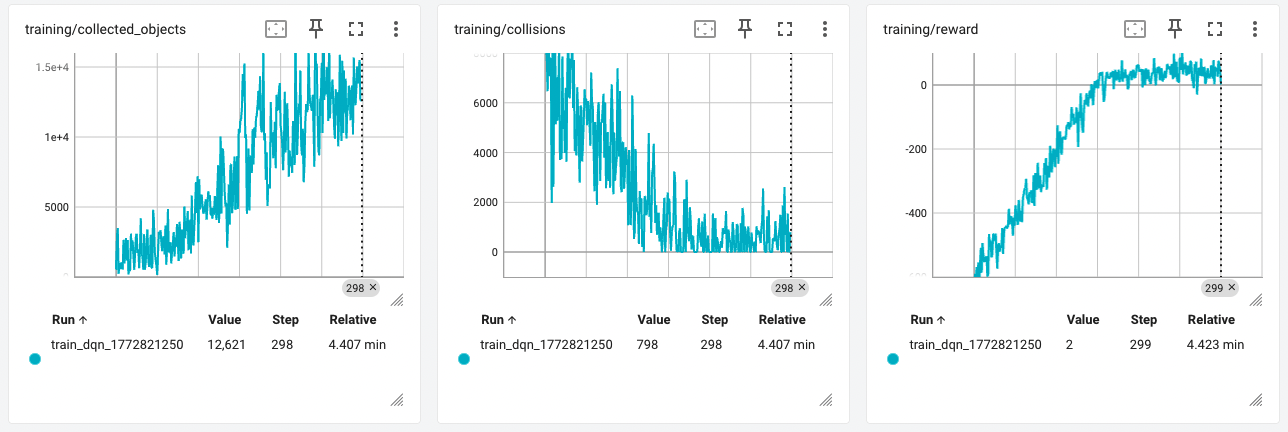
\includegraphics[width=\textwidth]{./img/collabsort_results.png}
    \captionof{figure}{Example of experimental results for a simulation of 300 episodes of 1000 timesteps each, with no reward changes between episodes. The evaluated metrics are the number of collected objects (left), the number of collisions between arms (center) and the cumulated episode reward (right).}
    \label{fig:collabsort_results}
\end{floating}

\section{Conclusion and perspectives}

Building from research at the crossroads of artificial intelligence, psychology and computational neuroscience, we developed a metacognitive artificial agent capable of assessing its own confidence levels and dynamically adjusting its decision-making accordingly. A dedicated testbed inspired by a human-robot collaboration project has been created to assess the agent's abilities and compare them to more standard approaches.

Future work will focus on refining and expanding the cognitive architecture to address broader aspects of metacognition, ultimately working toward more autonomous and flexible behavior in artificial agents.

%----------------------------------------------
% Bibliography
%----------------------------------------------

\begin{thebibliography}{99}

\bibitem{mileticNewModelDecision2021}
Steven Miletic, Russell J Boag, Anne C Trutti, Niek Stevenson, Birte U Forstmann, and Andrew Heathcote. A new model of decision processing in instrumental learning tasks. eLife, 10:e63055, January 2021.

\bibitem{radfordLLM}
Alec Radford et al., Improving Language Understanding by Generative Pre-Training, n. d.

\bibitem{suttonBartoRL}
Richard S. Sutton et Andrew G. Barto, Reinforcement Learning: An Introduction, Second edition, Adaptive Computation and Machine Learning Series (The MIT Press, 2018).

\bibitem{weiCoTreasoning2024}
Jason Wei, Xuezhi Wang, Dale Schuurmans, Maarten Bosma, Brian Ichter, Fei Xia, Ed H. Chi, Quoc V. Le, and Denny Zhou. Chain-of-thought prompting elicits reasoning in large language models. NIPS ’22, pages 24824–24837, Red Hook, NY, USA, April 2024. Curran Associates Inc.

\bibitem{botvinickRLfastslow}
Matthew Botvinick et al., Reinforcement Learning, Fast and Slow, Trends in Cognitive Sciences 23, n 5 (2019): 408‑22.

\bibitem{goldNeuralBasis2007}
Joshua I. Gold and Michael N. Shadlen. The Neural Basis of Decision Making. Annual Review of Neuroscience, 30(1):535–574, July 2007.

\bibitem{forstmannSSM2016}
B.U. Forstmann, R. Ratcliff, and E.-J. Wagenmakers. Sequential Sampling Models in Cognitive Neuroscience: Advantages, Applications, and Extensions. Annual Review of Psychology, 67(1):641–666, January 2016.

\bibitem{suriNNDopamine1999}
R.E.Suri and Wolfram Schultz, A Neural Network Model with Dopamine-Like Reinforcement Signal that Learns a Spatial Delayed Response Task. Neuroscience, 91(3):871–890, July 1999.

\bibitem{mnihDQN2015}
Mnih, V., Kavukcuoglu, K., Silver, D. et al. Human-level control through deep reinforcement learning. Nature 518, 529–533 (2015)

\bibitem{zilliModelingWMEM2008}
Eric A. Zilli et Michael E. Hasselmo, Modeling the Role of Working Memory and Episodic Memory in Behavioral Tasks, Hippocampus 18, n 2 (2008): 193‑209.

\bibitem{stolleOptionsRL2002}
Martin Stolle et Doina Precup, « Learning Options in Reinforcement Learning », in Abstraction, Reformulation, and Approximation, ed. by G. Goos et al., vol. 2371, éd. par Sven Koenig et Robert C. Holte, Lecture Notes in Computer Science (Springer Berlin Heidelberg, 2002).

\bibitem{baconOptionCritic2016}
Pierre-Luc Bacon et al., « The Option-Critic Architecture », arXiv:1609.05140, prépublication, arXiv, 3 décembre 2016.

\bibitem{KepecsDecisionConfidence2008}
Adam Kepecs, Naoshige Uchida, Hatim A. Zariwala, and Zachary F. Mainen. Neural correlates, computation and behavioural impact of decision confidence. Nature, 455(7210):227–231, September 2008

\bibitem{koechlinPROBE2012}
Anne Collins et Etienne Koechlin, Reasoning, Learning, and Creativity: Frontal Lobe Function and Human Decision-Making, PLoS Biology 10, n 3 (2012): e1001293.

\end{thebibliography}
\end{content}
\end{document}
